\begin{adjustwidth*}{}{-2.25in}
\textbf{{\large Exercises}}
\setlength{\columnsep}{25pt}
\begin{multicols*}{2}
\noindent Terms and Concepts \small
\begin{enumerate}[1)]
\item T/F: A solid of revolution is formed by revolving a shape around an axis.
\item In your own words, explain how the Disk and Washer Methods are related.
\item Explain the how the units of volume are found in the integral: if $A(x)$ has units of in$^2$, how does $\int A(x)\ dx$ have units of in$^3$?
\end{enumerate} 

\noindent {\normalsize Problems} \small

\noindent{\bf In Exercises 4--7, a region of the Cartesian plane is shaded. Use the Disk/Washer Method to find the volume of the solid of revolution formed by revolving the region about the $x$-axis.}

\begin{enumerate}[1),resume]
\item \begin{minipage}{\linewidth}\centering\includegraphics{figures/fig07_02_ex_04}\end{minipage}

\item \begin{minipage}{\linewidth}\centering\includegraphics{figures/fig07_02_ex_05}\end{minipage}

\item \begin{minipage}{\linewidth}\centering\includegraphics{figures/fig07_02_ex_06}\end{minipage}

\item \begin{minipage}{\linewidth}\centering\includegraphics{figures/fig07_02_ex_07}\end{minipage}
\end{enumerate}

\noindent{\bf In Exercises 8-11, a region of the Cartesian plane is shaded. Use the Disk/Washer Method to find the volume of the solid of revolution formed by revolving the region about the $y$-axis.}

\begin{enumerate}[1),resume]
\item \begin{minipage}{\linewidth}\centering\includegraphics{figures/fig07_02_ex_08}\end{minipage}

\item \begin{minipage}{\linewidth}\centering\includegraphics{figures/fig07_02_ex_09}\end{minipage}

\item \begin{minipage}{\linewidth}\centering\includegraphics{figures/fig07_02_ex_10}\end{minipage}
\end{enumerate}

%------------------------------------------
% END OF EXERCISES ON FIRST PAGE
%------------------------------------------
\end{multicols*}
\end{adjustwidth*}

\clearpage

\begin{adjustwidth*}{}{-2.25in}
\setlength{\columnsep}{25pt}
\begin{multicols*}{2}\small

\begin{enumerate}[1),start=11]
\item \begin{minipage}{\linewidth}\centering\includegraphics{figures/fig07_02_ex_11}\end{minipage}

(Hint: Integration By Parts will be necessary, twice. First let $u = \arccos^2x$, then let $u=\arccos x$.)
\end{enumerate}

\vspace{.25cm}

\noindent{\bf In Exercises 12--17, a region of the Cartesian plane is described. Use the Disk/Washer Method to find the volume of
the solid of revolution formed by rotating the region about each of the given axes.}

\begin{enumerate}[1),resume]
\item Region bounded by: $y=\sqrt{x}$, $y=0$ and $x=1$.

Rotate about:

\noindent%
\begin{minipage}[t]{.5\linewidth}
\begin{enumerate}
\item		the $x$-axis
\item		$y=1$
\end{enumerate}
\end{minipage}
\begin{minipage}[t]{.5\linewidth}
\begin{enumerate}\addtocounter{enumii}{2}
\item		the $y$-axis
\item		$x=1$
\end{enumerate}
\end{minipage}

\item Region bounded by: $y=4-x^2$ and $y=0$.

Rotate about:

\noindent%
\begin{minipage}[t]{.5\linewidth}
\begin{enumerate}
\item		the $x$-axis
\item		$y=4$
\end{enumerate}
\end{minipage}
\begin{minipage}[t]{.5\linewidth}
\begin{enumerate}\addtocounter{enumii}{2}
\item		$y=-1$
\item		$x=2$
\end{enumerate}
\end{minipage}

\item The triangle with vertices $(1,1)$, $(1,2)$ and $(2,1)$.

Rotate about:

\noindent%
\begin{minipage}[t]{.5\linewidth}
\begin{enumerate}
\item		the $x$-axis
\item		$y=2$
\end{enumerate}
\end{minipage}
\begin{minipage}[t]{.5\linewidth}
\begin{enumerate}\addtocounter{enumii}{2}
\item		the $y$-axis
\item		$x=1$
\end{enumerate}
\end{minipage}

\item Region bounded by $y=x^2-2x+2$ and $y=2x-1$.

Rotate about:

\noindent%
\begin{minipage}[t]{.5\linewidth}
\begin{enumerate}
\item		the $x$-axis
\item		$y=1$
\end{enumerate}
\end{minipage}
\begin{minipage}[t]{.5\linewidth}
\begin{enumerate}\addtocounter{enumii}{2}
%\item		the $y$-axis
\item		$y=5$
\end{enumerate}
\end{minipage}

\item Region bounded by $y=1/\sqrt{x^2+1}$, $x=-1$, $x=1$ and the $x$-axis.

Rotate about:

\noindent%
\begin{minipage}[t]{.5\linewidth}
\begin{enumerate}
\item		the $x$-axis
\item		$y=1$
\end{enumerate}
\end{minipage}
\begin{minipage}[t]{.5\linewidth}
\begin{enumerate}\addtocounter{enumii}{2}
%\item		the $y$-axis
\item		$y=-1$
\end{enumerate}
\end{minipage}

\item Region bounded by $y=2x$, $y=x$ and $x=2$.

Rotate about:

\noindent%
\begin{minipage}[t]{.5\linewidth}
\begin{enumerate}
\item		the $x$-axis
\item		$y=4$
\end{enumerate}
\end{minipage}
\begin{minipage}[t]{.5\linewidth}
\begin{enumerate}\addtocounter{enumii}{2}
\item		the $y$-axis
\item		$x=2$
\end{enumerate}
\end{minipage}

\end{enumerate}

\noindent{\bf In Exercises 18--21, a solid is described. Orient the solid along the $x$-axis such that a cross-sectional area function $A(x)$ can be obtained, then find the volume of the solid.}

\begin{enumerate}[1),resume]
\item A right circular cone with height of 10 and base radius of 5. \label{ex_07_02_ex_18}

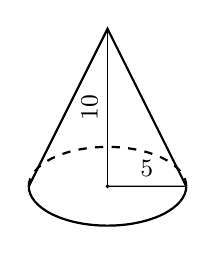
\begin{tikzpicture}[scale=.5]
\begin{scope}[xscale=2]
%\draw [thick](0,0) circle (1);
\draw [thick] (-1,0) arc (180:360:1);
\draw [thick,dashed] (1,0) arc (0:180:1);
\end{scope}

\draw [fill=black] (0,0) circle (1pt) -- node [pos=.5,above] {\small 5} (2,0);
\draw (0,0) -- node [pos=.5,rotate=90,above] {\small 10} (0,4);
\draw [thick] (-2,0) -- (0,4)-- (2,0);
\end{tikzpicture}

\item A skew right circular cone with height of 10 and base radius of 5. (Hint: all cross-sections are circles.)

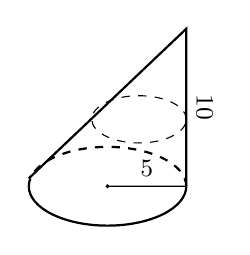
\begin{tikzpicture}[scale=.5]
\begin{scope}[xscale=2]
%\draw [thick](0,0) circle (1);
\draw [thick] (-1,0) arc (180:360:1);
\draw [thick,dashed] (1,0) arc (0:180:1);
\draw [dashed] (.4,1.7) circle (.6);
\end{scope}

\draw [fill=black] (0,0) circle (1pt) -- node [pos=.5,above] {\small 5} (2,0);
%\draw (0,0) -- node [pos=.5,rotate=90,above] {\small 10} (0,4);
\draw [thick] (-2,0.2) -- (2,4)-- node [pos=.5,rotate=-90,above] {\small 10}(2,0);
\end{tikzpicture}

\item A right triangular cone with height of 10 and whose base is a right, isosceles triangle with side length 4.

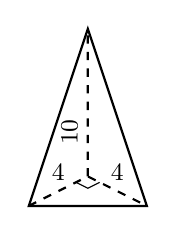
\begin{tikzpicture}[scale=.75]
\draw [thick](-1,0) -- (1,0) -- (0,3)--cycle;
\draw [thick,dashed] (-1,0) --  node [pos=.5,above] {\small 4} (0,.5) -- node [pos=.5,above] {\small 4} (1,0)
											(0,.5)-- node [pos=.3,above,rotate=90] {\small 10} (0,3);
\draw (-.2,.4) -- (0,.3) -- (.2,.4);
\end{tikzpicture}

\item A solid with length 10 with a rectangular base and triangular top, wherein one end is a square with side length 5 and the other end is a triangle with base and height of 5.

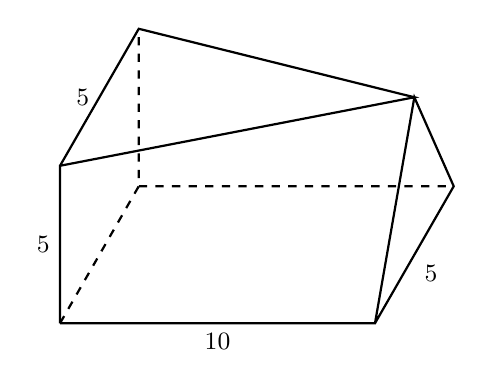
\begin{tikzpicture}[x={(1,0)},z={(0,1)},y={(.5,.87)},scale=.4]

\draw [thick] (0,0,0) -- node[pos=.5,below] {\small 10} (10,0,0) -- (10,2.5,5) -- (10,5,0) -- node [pos=.5,below right] {\small 5} (10,0,0)
							(0,0,0) -- node [pos=.5,left] {\small 5} (0,0,5) -- (10,2.5,5) -- (0,5,5) -- node [pos=.5,left] {\small 5} (0,0,5);
							
\draw [thick,dashed] (0,0,0) -- (0,5,0) -- (0,5,5)
										(0,5,0) -- (10,5,0);



\end{tikzpicture}

\end{enumerate}

%---------------------------------------------
% END OF EXERCISES ON SECOND PAGE
%---------------------------------------------
\end{multicols*}
\end{adjustwidth*}

\afterexercises